
\section{Information Flow Theory} 
The following sections give a brief introduction to the general notion of \emph{security} in regards to the concept of information in computational systems.
Building upon this, we then focus specifically on the key concepts of non-interference and declassification as they relate to the notion of information flow.
\subsection{Security models and policies}
Many modern computational systems will at some point have to handle certain kinds of information, which must never be accessible to an \emph{unauthorized} entity.
A popular description for a system, which keeps its information from leaking to the outside or any unintended entity/process can be found in the term of a  \emph{secure} system.
In this context, ``security'' or ``secure information flow'' means, that "no unauthorized flow of information is possible" \cite{lattice_model_security}.

While such a general definition may be relatively easy to arrive at, actually \emph{enforcing} the necessary constraints on the numerous information pipelines and flows within even a single program is often no easy task at all. 
In order to properly define which information may flow in what way within a part of a program or between programs, a common approach is to specify the individual components, between which a flow of information may occur and consequently assigning certain security \emph{levels} to these individual constituents. This approach can for example be found in \cite{lattice_model_security} by \citeauthor{lattice_model_security}, in which the concept of \emph{security classes} \(SC\) is introduced. These classes can then be bound to any information receptacles or ``objects'' in order to denote their respective security clearance.
\todo{This chapter is way too short at the moment.}
\todo{Mention, that the lattice model is very widespread and fundamental. Tie into this later aswell. (Public/Private can be seen as a binary lattice model.)}
\subsection{Non-interference and Declassification}
\label{ref:Declass_and_Inter}
An important concept in terms of secure systems that can be operated by multiple users either simultaneously or sequentially, is the concept of \emph{non-interference}.
\begin{quotation}
    One group of users, using a certain set of commands, is noninterfering with another group of users if what the first group does with those commands has no effect on what the second group of users can see
\end{quotation}

To explain this concept in terms of our problem domain of PGP servers, let us assume running instance of HAGRID which is publicly accessible. Let us further assume that there are two users \(u1\) and \(u2\) that are interacting with the server at the same time. Additionally, each user holds a certain set of keys:


\(
    u1 := \begin{cases}
        k1 = \text{Key(id1,id2)} \\
        k2 = \text{Key(id3,id4)}
    \end{cases}
    \) and \, \(
    u2 := \begin{cases}
        k3 = \text{Key(id5,id6)} \\
        k4 = \text{Key(id7,id8)}
    \end{cases}
    \)

Based on this, we can image the following, highly simplified interaction between the two users and HAGRID
\begin{figure}[h]
    \label{fig:example}
    \centering
    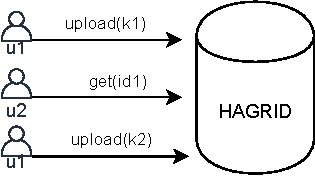
\includegraphics{images/non_interference.pdf}
    \caption{A non-interfering interaction}
\end{figure}

The second call of \(u2\) in this sequence is a key request for identity \(id1\) which belongs to the previously uploaded key \(k1\). Yet, because the identity had not been verified when \(u2\) issued its key request, the resulting response will be empty. That means, that the actions of \(u1\) hat no effect \emph{at all} on the experience of \(u2\). 
As a matter of fact, based on the interactions with HAGRID alone, \(u2\) has no way of identifying whether there even \emph{is} another user currently interacting with the same system. 
In contrast to that, let us assume that this sequence of interactions is continued in the following way: 
\begin{figure}[h]
    \label{fig:example}
    \centering
    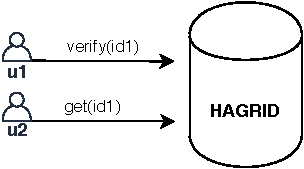
\includegraphics{images/interfering.pdf}
    \caption{The interaction has become interfering}
\end{figure}

The second \(get\) request now yields a different response as before. Instead of an empty response, \(u2\) now receives a key with an identity. This change in behaviour was caused by \(u1\) issuing a verification for \(id1\). Therefore, the actions of \(u1\) were able to influence the sequence of interactions between \(u2\) and HAGRID, which causes this interaction to no longer be \emph{non-interfering}.
\\ \\

\paragraph{Definition of non-interference by \citeauthor{Goguen_Meseguer_82}}
A more formal definition of non-interference is given by \citeauthor{Goguen_Meseguer_82} in \citetitle{Goguen_Meseguer_82}, which is also the paper that initially popularized the notion of non-interference. 
In order to give a brief summary of their definition of non-interference, let us first introduce the central terms on which their definition relies. From here on, let \(Q\) denote some abstract system, which can be approximately modeled as some state machine \(M = \{U,S,C,\text{Out}\}\). 
In this context, let \(U\) be a set whose elements denote the users of \(Q\). Additionally, let \(S\) be the set of abstract states of \(M\), while \(C\) denotes the set of ``commands'' that may cause a state transition in \(M\). Finally, let \(\text{Out}\) refer to the set of all ``outputs'' that \(Q\) may generate. 
Given these foundational definitions, \citeauthor{Goguen_Meseguer_82} proceed to define a function \(p\): 

Given a subset \(G\) of all users \(U\) and some subset \(A\) of state altering commands \(C\), let \(w\) be in \((U \times C)^*\). That is, \(w\) is an ordered sequence of pairs consisting of a user and an associated command. 

Finally, let \(p_G(w)\) be equal to \(w\) excluding any pairs \((u,c)\), where \(u \in G\). Similarly, let \(p_A(w)\) be equal to \(w\) excluding any pairs \((u,c)\) where \(c \in A\). In combination, let \(p_{G,A}\) be equal to \(w\) excluding any pairs \((u,c)\) where \(u \in G\) and \(c \in A\).
From there, \citeauthor{Goguen_Meseguer_82} then directly derive three notions of non-interference:
\begin{enumerate}
    \item Non-interference between two sets of users: Given a state machine \(M\) and two sets of users \(G\) and \(G'\), we let \(G :\mid G'\) denote that \(G\) and \(G'\) are non-interfering, iff \[ 
        [[\;w\;]]_u = [[\;p_G(w)\;]]_u  
    \]
    That is, they are only non-interfering if the outputs caused by \(w\) are equal to those produced by the subsequence of \(w\) excluding any element involving a user from \(G\).
    \item Non-interference between an ability \(A\) and a set of users \(G\): Given a state machine \(M\), we let \(A :\mid G\) denote that \(A\) and \(G\) are non-interfering, iff \[
        [[\;w\;]]_u = [[\;p_A(w)\;]]_u  
    \]
    That is, they are only non-interfering if the outputs caused by \(w\) are equal to those produced by the subsequence of \(w\) excluding any element involving an ability from \(A\).
    \item Non-interference between a set of users \(G\) with ability \(A\) and another set of users \(G'\): Given a state machine \(M\), we let \(A,G :\mid G'\) denote that no user from \(G\) with ability \(A\) interferes with users from \(G'\), iff \[
        [[\;w\;]]_u = [[\;p_{G,A}(w)\;]]_u   
    \]
    That is, they are only non-interfering if the outputs caused by \(w\) are equal to those produced by the subsequence of \(w\) excluding all elements involving a user from \(G\) and ability from \(A\).
\end{enumerate}



Note that all of the definitions above describe purely \emph{static} non-interference policies. That is, the non-interference policy must always hold and thus never allows any sets of users and abilities to interfere \emph{at all}. 

Given this definition of non-interference, it can be trivially concluded that strict enforcement of this principle would render most information systems practically unusable.
To mitigate the strictness of these definitions, \citeauthor{Goguen_Meseguer_82} further introduce the notion of \emph{conditional non-interference}, which encodes the notion that the definitions given above must only hold under some condition \(P\): \[
     G,A :\mid G' \; \text{if } P 
\]

Applied to Hagrid: Let \(U\) be the set of all users. Let \(G,G' \subset U\) be two sets of users that are both accessing the same key \(K\). Let \(u \in G\) and \(c\) be the set of state altering operations provided by Hagrid (Verify, Revoke): 
\[
    \forall u,c \;.\; \{u\}, \{c\} :\mid G' \text{ if not } \text{CHECK}(u,c,K),
\]
where CHECK\((u,c,K)\) describes whether \(u\) can use \(c\) to affect the state of \(K\) in any meaningful way.

That is, given some key K, we guarantee that a user \(u\) does not interfere with any other user that operates on the same key as long as \(u\) lacks the ability to verify or revoke identities associated with \(K\). 
In return, that also means that we explicitly permit interference by supporting declassification of formerly confidential information in such cases, where it is permissible for a user to affect the privacy state of some key \(K\).

As \citeauthor{declass_dim_prin} explain in their paper \citetitle{declass_dim_prin}, the core issue therefore lies with ensuring that the release of information in these instances is actually \emph{safe}. That is, that such a system never accidentally declassifies more information than it ought to, as that would consequently also violate its non-interference policies.
The main challenge that one faces when trying to \emph{verify} whether Hagrid adheres to these policies, is that the set of theoretically visible identities is constantly changing and strongly depends on dynamic runtime values within the Hagrid system. 
While there exist some approaches like the one laid out in \citetitle{Lourenco_Caires_15} by \citeauthor{Lourenco_Caires_15}, which are based on Dependent Type Theory and allow one to formulate Information Flow types that depend on runtime values, these approaches are relatively novel and unexplored.

In the following chapter, we instead present an approach to ensure the safe declassification of sensitive information during runtime that utilizes the notion of state machines similarly to \citeauthor{Goguen_Meseguer_82}. We then extend the approach in such a way, as to allow us to specify exactly what sensitive information is declassifiable (or potentially reclassifiable) by Hagrid based on the input of the system.

